 \section{Some global aspects of the higher Kac-Moody factorization algebras}

A compelling aspect of factorization algebras is that they are local-to-global objects,
and hence the global sections---the factorization homology---can contain quite interesting information.
For instance, in the case of a one-dimensional locally constant factorization algebra, the global sections along a circle encodes the Hochschild homology of the corresponding associative algebra. 
In the complex one-dimensional situation, the factorization homology along Riemann surfaces is closely related to the conformal blocks of the associated vertex algebra. 

In the first part of this section, we direct our attention to a class of complex manifolds called {\em Hopf manifolds},
whose underlying smooth manifold has the form $S^1 \times S^{2d-1}$.
They provide a natural generalization of elliptic curves, and hence to generalizations of interesting phenomena from chiral CFT in complex dimension one.
In particular, the factorization homology on Hopf manifolds serves as a natural home for characters of representations of the sphere algebra~$\Tilde{\fg}_{d,\theta}^\bullet$.
We demonstrate that by identifying the factorization homology with the Hochschild homology of~$\Tilde{\fg}_{d,\theta}^\bullet$.

In the next section, we provide examples of such characters using field theory.
In physical terms, the factorization homology is related to the partition function of $\sG$-equivariant holomorphic field theories, such as the higher dimensional $\beta\gamma$ and $bc$ systems.
We compute the partition functions on these Hopf manifolds, which are close cousins to superconformal indices, 
and give a concise description in terms of Hochschild homology, in Proposition~\ref{prop: hopf}. 
\brian{more on index/character}

Finally, we return to the LMNS variants of the twisted higher Kac-Moody factorization algebra that exist on other closed $d$-folds and assert a relationship to the ordinary Kac-Moody algebra on Riemann surfaces. 

\subsection{Hopf manifolds and Hochschild homology}

\owen{add comment}

\subsubsection{Overview of Hopf manifolds}

Recall that for every complex number $q$ such that $0< |q| < 1$, 
there is a natural action of $\ZZ$ on the punctured plane $\CC^\times$ where $n \cdot z = q^n z$.
We will denote this multiplicative action with the succinct notation $q^\ZZ$.
The quotient space $\CC^\times/q^\ZZ$ is then an elliptic curve,
and the punctured unit disk $\{0< |q|<1\}$ parametrizes elliptic curves in a convenient way.

This story admits an obvious higher dimensional generalization, first explored by Hopf~\cite{Hopf}.

\begin{dfn}
Let $d$ be a positive integer.
Let ${\bf q} = (q_1,\ldots, q_d)$ be a $d$-tuple of complex numbers where $0 < |q_i| < 1$ for $i = 1, \ldots, d$. 
The $d$-dimensional {\em Hopf manifold} $X_{\bf q}$ is the quotient of punctured affine space $\CC^d \setminus \{0\}$ by the multiplicative action of~$\ZZ$:
\[
X_{\bf q} = \left. \left(\CC^d \setminus \{0\}\right) \right/ {\bf q}^\ZZ.  
\]
In other words, we quotient by the equivalence relation
\[
(z_1,\ldots,z_d) \sim (q_1^{n} z_1, \ldots,q_d^{n} z_d)
\]
where $n$ runs over $\ZZ$.
\end{dfn}

\owen{I removed the $2 \pi i$ factors from the exponent, if that's OK.}

We denote the obvious quotient map by $p_{\bf q} : \CC^d \setminus \{0\} \to X_{\bf q}$. 
It is a straightforward exercise to check that $X_{\bf q}$ is diffeomorphic to $S^{2d-1} \times S^1$ as smooth manifolds;
the clearest situation is where $q_1 = q_2 = \cdots = q_d$,
which is the most direct generalization of elliptic curves.

\begin{rmk}
By definition, a Hopf manifold of dimension $d$ is a complex manifold diffeomorphic to $S^{2d-1} \times S^1$. 
Our arguments below extend with only a little extra effort to an arbitrary Hopf manifold, 
but this class is interesting and easy to work with.
Note that for $d>1$, $H^{2}_{dR} (X_{\bf q}) = 0$ and so Hopf manifolds are {\em not} K\"{a}hler in complex dimensions bigger than one. 
\end{rmk}

A key fact for us is that the Dolbeault complex of a Hopf manifold admits a small model.

\begin{lem}\label{lem:tanre}
For any Hopf manifold $X_{\bf q}$, there is a quasi-isomorphic inclusion of bigraded complexes
\[
(\CC[a, b, \alpha, \beta], \delta) \hookrightarrow (\Omega^{*,*}(X_{\bf q}),\dbar)
\]
where the generator $a$ has bidegree $(1,1)$, $b$ has bidegree $(d,d-1)$, $\alpha$ has bidegree $(0,1)$, and $\beta$ has bidegree $(1,0)$, and where $\delta(a) = 0$, $\delta(b) = a^{d}$, $\delta(\alpha) = 0$, and $\delta(\beta) = a$.
Here $\dbar$ and $\delta$ both have bidegree~$(0,1)$.
\end{lem}

We borrow this claim from chapter 4 of~\cite{Tanre}, particularly example 4.63,
and simply sketch the main points.
Notably, a Hopf manifold is the total space of a fibration
\[
S^1 \times S^1 \to X_{\bf q} \to \CC\PP^{d-1}.
\]
Topologically, this fibration is the product of a circle with the Hopf fibration $S^1 \to S^{2d+1} \to \CC\PP^{d-1}$. 
Each torus fiber can be equipped with the complex structure of some elliptic curve, so that the fibration is holomorphic with respect to the natural complex structures on $X_{\bf q}$ and~$\CC\PP^{d-1}$.
Both projective space and an elliptic curve are K\"ahler and hence admit small models, 
following~\cite{DGMS}.
As the Hopf manifold is a fibration, one obtains a model for its Dolbeault complex by twisting the differential on the tensor product of those models.
The lemma above specifies the relevant twisting.

It is also possible to obtain a small model for the {\em de Rham} complex by a further twisting. 
(See Theorem 4.70 of~\cite{Tanre}.)
For the Hopf manifold, however, life is particularly simple.

\begin{lem}[Example 4.72, \cite{Tanre}]
For $X_{\bf q}$ a Hopf manifold,
the Dolbeault cohomology coincides with the de Rham cohomology $H^*(S^1) \otimes H^*(S^{2d-1})$.
Moreover, the complex $(\CC[a, b, \alpha, \beta], \delta)$ is also a de Rham model and hence is quasi-isomorphic to the de Rham complex.
\end{lem}

Our primary interest, however, is in the $(0,*)$-forms.
The complex $\Omega^{0, *}(X_{\bf q})$ sits inside $\Omega^{*, *}(X_{\bf q})$ as a summand,
and similarly the complex $\CC[\alpha]$ sits inside $(\CC[a, b, \alpha, \beta], \delta)$ as a summand,
yielding the following result.

\begin{lem}
There is a quasi-isomorphic inclusion 
\[
(\CC[\alpha], 0) \hookrightarrow (\Omega^{0,*}(X_{\bf q}), \dbar)
\]
induced by the inclusion in lemma~\ref{lem:tanre}.
\end{lem}

Note that the source is precisely the small model for the Dolbeault complex $\Omega^{0, *}(E)$ of an elliptic curve,
and---more importantly---for the de Rham complex of a circle.

\begin{eg}
Consider 
the $(0,1)$-form 
\[
\dbar (\log |z|^2) = \sum_i \frac{z_i\d \zbar_i}{|z|^2} 
\]
on $\CC^d \setminus \{0\}$.
It is $\ZZ$-invariant, and hence descends along the map $p_{\bf q} : \CC^d \setminus 0 \to X$
when ${\bf q} = (q,\ldots,q)$ with $|q| < 1$.
The descended form thus provides an explicit Dolbeault representative for~$\alpha$.
\end{eg}

Finally, the complex  $\Omega^{d, *}(X_{\bf q})$ will appear later. 
We note that the corresponding subcomplex inside $(\CC[a, b, \alpha, \beta], \delta)$ is the summand
\[
\CC b \oplus \CC a^{d-1} \beta \to \CC b \alpha \oplus \CC a^{d} \oplus \CC a^{d-1} \alpha \beta \to \CC a^{d} \alpha,
\]
concentrated between bidegrees $(d,d-1)$ and $(d,d+1)$.
As $\delta(a^{d-1} \alpha \beta) = a^d \alpha$, and $\delta(a^{d-1} \beta) = a^d$, 
we see that the cohomology is spanned by $b$ in bidegree $(d,d-1)$ and $b \alpha$ in bidegree~$(d,d)$.

%For any $d$ and tuple $(q_1,\ldots, q_d)$ as above, we see that as a smooth manifold there is a diffeomorphism $X_{\bf q} \cong S^{2d-1} \times S^1$. 
%Indeed, the radial projection map $\CC^d \setminus \{0\} \to \RR_{>0}$ defines a smooth $S^{2d-1}$-fibration over $\RR_{>0}$. 
%Passing to the quotient, we obtain an $S^{2d - 1}$-fibration 
%\[
%X_{\bf q} \to \left. \RR_{>0} \right/ \left(r \sim \lambda^{\ZZ} \cdot r \right) \cong S^1 .
%\]
%Here, $\lambda = (|q_1|^2 + \cdots + |q_d|^2)^{1/2} > 0$. 
%Since there are no non-trivial $S^{2d-1}$ fibrations over $S^1$ we obtain $X_{\bf q} = S^{2d-1} \times S^1$ as smooth manifolds. 

\subsubsection{Current algebras on Hopf manifolds}

For any choice of ${\bf q} = (q_1,\ldots,q_d)$, we have the local Lie algebra $\sG_{X_{\bf q}} = \Omega^{0,*}(X_{\bf q}, \fg)$, and the corresponding Kac-Moody factorization algebra obtained by the enveloping factorization algebra $\UU\sG_{X_{\bf q}}$.
A choice of invariant polynomial $\theta \in \Sym^{d+1}(\fg^*)^\fg$ defines a $\CC[K]$-linear twisted factorization enveloping algebra $\UU_{\theta}(\sG_{X_{\bf q}})$.  
Our first result is a computation of the global sections of this factorization algebra.  

\begin{prop}
\label{prop: hopf}
Let $X_{\bf q}$ be a Hopf manifold and let $\theta \in \Sym^{d+1}(\fg^*)^\fg$ be an $\fg$-invariant polynomial of degree $(d+1)$. 
There is a quasi-isomorphism of $\CC[K]$-modules
\[
\UU_\theta (\sG) (X_{\bf q}) \xto{\simeq} \Hoch_*(U \fg)[K] .
\]
\end{prop}

\begin{proof}
Fix ${\bf q}$ and write simply $X$ for $X_{\bf q}$ and $\sG$ for $\sG_X$. 
We first consider the untwisted case, with $\theta = 0$, where the statement reduces to $\UU\sG(X) \simeq \Hoch_*(U \fg)$.
The factorization homology on the left hand side is computed by
\[
\UU \sG (X) = \clieu_*(\Omega^{0,*}(X) \tensor \fg) .
\]
Our goal is to compute the Lie algebra homology of the dg Lie algebra $\Omega^{0,*}(X) \tensor \fg$.  

We know that $H^{0,*}(X) \cong \CC[\alpha]$ where $\alpha$ has degree 1, by the arguments above.
Hodge theory will let us produce a quasi-isomorphism $(\Omega^{0,*}(X), \dbar) \to \CC[\alpha]$.
Indeed, any Hermitian metric on $X$ determines an adjoint $\dbar^*$ to $\dbar$ and hence a Dolbeault Laplacian $\Delta_{\dbar} = [\dbar,\dbar^*]$.
Denote by $\sH^{0,*}_{\dbar}(X)$ the graded vector space of harmonic $(0,*$-forms, i.e., those annihilated by $\Delta_{\dbar}$. 
In light of lemma~\ref{lem:tanre}, the orthogonal projection determines a quasi-isomorphism
\beqn\label{hopfquasi}
\pi_{\sH}^{0,*} : \left(\Omega^{0,*}(X), \dbar \right) \xto{\simeq} \sH^{0,*}_{\dbar}(X) \cong \CC[\alpha].
\eeqn
Tensoring with $\fg$, we obtain a quasi-isomorphism 
\beqn\label{Lieproj}
\pi_{\sH}^{0,*} \otimes \id_\fg :\sG (X) \to \fg[\alpha]
\eeqn
of dg Lie algebras, where the target has trivial differential.

\begin{rmk}\label{rmk: hpl1}
In fact, by ellipticity, the orthogonal projection extends to a deformation retraction of dg Lie algebras
\begin{equation*}\label{contraction}\tag{$\ast$}
  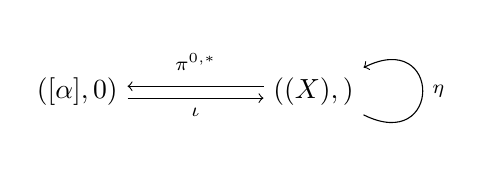
\begin{tikzpicture}[baseline=(L.base),anchor=base,->,auto,swap]
     \path node (L) {$(\fg[\alpha],0)$} ++(3,0) node (M) {$(\sG (X), \dbar)$} 
     (M.mid) +(0,.075) coordinate (raise) +(0,-.075) coordinate (lower);
     \draw (L.east |- lower) to node {$\scriptstyle \iota$} (M.west |- lower);
     \draw (M.west |- raise) to node {$\scriptstyle \pi_{\sH}^{0,*} $} (L.east |- raise);
     \draw (M.south east) ..controls +(1,-.5) and +(1,.5) .. node {$\scriptstyle \eta$} (M.north east);
  \end{tikzpicture}\end{equation*}
The map $\iota$ is the inclusion of harmonic forms. 
The operator $\eta$ is constructed from the Green's function $p(z,w) \in \Omega^{d,*}(X \times X)$ of the $\dbar$ operator on $X$ which satisfies 
\[
\dbar_w p(z,w) = \omega_{diag}
\]
where $\omega_{diag}$ is the volume form along the diagonal in $X \times X$. 
The homotopy $\eta$ is defined by
\[
(\eta \alpha)(z) = \int_{w \in X} p(z,w) \alpha(w) .
\]
It satisfies the homotopy retraction condition
\[
\iota \circ \pi - \id_{\sG} = \dbar \eta +\eta \dbar = [\dbar,\eta]  .
\]
\end{rmk}


%Here, we view $\CC[\epsilon,\delta]$ as a cochain complex with zero differential. 


Applying Chevalley-Eilenberg chains to Equation (\ref{Lieproj}), we obtain the following quasi-isomorphism for the global sections of the untwisted Kac-Moody factorization algebra:
\beqn\label{hopfquasi3}
\begin{tikzcd}
\clieu_*(\pi_{\sH}^{0,*}) : \displaystyle \UU\sG (X) = \clieu_*(\Omega^{0,*}(X , \fg)) \ar[r,"\simeq"] &\clieu_*(\CC[\epsilon] \tensor \fg) .
\end{tikzcd}
\eeqn
Unpacking the right hand side, we have
\[
\clieu_*(\CC[\alpha] \tensor \fg) = \clieu_*(\fg \oplus \fg[-1]) = \clieu_*(\fg, \Sym (\fg^{ad})),
\] 
where $\Sym(\fg^{ad})$ is the symmetric product of the adjoint representation of $\fg$. 
By the Poincar\'{e}-Birkoff-Witt theorem, there is an isomorphism of vector spaces $\Sym(\fg) \cong U \fg$, so we can write view this cochain complex as~$\clieu_*(\fg, U \fg^{ad})$.

Any $U(\fg)$-bimodule $M$ is automatically a module for the Lie algebra $\fg$ by the formula $x \cdot m = xm - mx$ where $x \in \fg$ and $m \in M$.
Moreover, for any such bimodule there is a quasi-isomorphism of cochain complexes 
\[
\clieu_*(\fg, M) \xto{\simeq} {\rm Hoch}_*(U\fg, M) 
\]
which is induced from the inclusion of $\fg \hookrightarrow U \fg$. 
(See, for instance, Theorem 3.3.2 of~\cite{LodayCyclic}.)
Applied to the bimodule $M = U\fg$ itself we obtain a quasi-isomorphism 
\[
\clieu_*(\fg , U\fg^{ad}) \xto{\simeq} {\rm Hoch}(U\fg).
\]
The right hand side is the Hochschild homology of $U\fg$ with values in $U\fg$ equipped with the standard bimodule structure. 
Composing with the quasi-isomorphism (\ref{hopfquasi3}) we obtain a quasi-isomorphism $\UU\sG(X) \xto{\simeq} \Hoch(U\fg)$, as desired.

We now consider the twisted case. 
Let $\theta$ be a nontrivial degree $(d+1)$ invariant polynomial on $\fg$. 
The factorization homology is then 
\[
\UU_\theta (\sG)(X) = \left(\Sym(\Omega^{0,*}(X) \tensor \fg)[K] , \dbar + \d_{CE} + K \cdot \d_\theta\right) .
\]
We wish to show that this cochain complex admits a quasi-isomorphism to $\Hoch_*(U \fg)[K]$.
The twisted complex is a $K$-linear deformation of the ordinary Lie algebra homology of $\sG(X)$. 
In particular, it does not follow that the orthogonal projection (\ref{Lieproj}) defines a quasi-isomorphism to $\Hoch_*(U \fg)[K]$.
In order to find an explicit quasi-isomorphism, we appeal to the homological perturbation lemma.
For more details on this result, see Section 2.5 of \cite{OwenThesis}. 

In the untwisted case, upon tensoring with $\CC[K]$, Remark \ref{rmk: hpl1} implies that we have a deformation retraction of cochain complexes
\begin{equation*}\tag{$\ast$}
  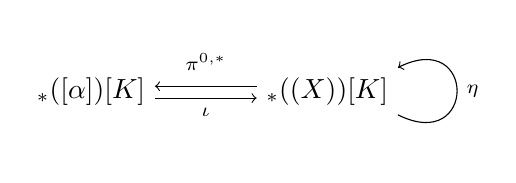
\begin{tikzpicture}[baseline=(L.base),anchor=base,->,auto,swap]
     \path node (L) {$\clieu_*(\fg[\alpha])[K]$} ++(3,0) node (M) {$\clieu_*(\sG (X))[K]$} 
     (M.mid) +(0,.075) coordinate (raise) +(0,-.075) coordinate (lower);
     \draw (L.east |- lower) to node {$\scriptstyle \iota$} (M.west |- lower);
     \draw (M.west |- raise) to node {$\scriptstyle \pi_{\sH}^{0,*} $} (L.east |- raise);
     \draw (M.south east) ..controls +(1,-.5) and +(1,.5) .. node {$\scriptstyle \eta$} (M.north east);
  \end{tikzpicture}\end{equation*}
  
To obtain the twisted complex, we turn on the deformation $K \cdot \d_\theta$ on the left-hand side. 
The homological perturbation lemma provides formulas for the resulting deformations of the projection, inclusion, and homotopy maps.
Explicitly, these formulas involve the formal inverse to the operator $\id_{\sG} - K \d_\theta \eta$ defined by
\[
(\id_{\sG} - K \d_\theta \eta)^{-1} = \sum_{n \geq 0} \frac{K^n}{n!} (\d_\theta \eta)^n  .
\] 
Note that acting on a particular element in the symmetric algebra~$\Sym(\Omega^{0,*}(\Omega^{0,*}(X) \tensor \fg[1])$ this formula is well-defined since only finitely many terms appear in the sum. 

With this operator in hand, we define the maps
\begin{eqnarray*}
\widetilde{\pi}^{0,*}_{\sH} & = & \pi + K \cdot \pi \circ (\id_{\sG} - K \d_\theta \eta)^{-1} \circ \d_\theta \circ \eta, \\
\widetilde{\eta} & = & \eta + K \cdot \eta \circ (\id_{\sG} - K \d_\theta \eta)^{-1} \circ \d_\theta \circ \eta .
\end{eqnarray*}
Note that modulo $K$ these reduce to the original maps above. 
The inclusion map $\iota$ and the differential on $\clieu_*(\fg[\alpha])$ do not get deformed in our situation because the perturbed piece of the differential $\d_{\theta}$ vanishes identically on the harmonic forms. 
The homological perturbation lemma implies that the resulting diagram
\begin{equation*}\tag{$\ast$}
  \begin{tikzpicture}[baseline=(L.base),anchor=base,->,auto,swap]
     \path node (L) {$\clieu_*(\fg[\alpha])[K]$} ++(3,0) node (M) {$\UU_\theta (\sG)(X) $} 
     (M.mid) +(0,.075) coordinate (raise) +(0,-.075) coordinate (lower);
     \draw (L.east |- lower) to node {$\scriptstyle \iota$} (M.west |- lower);
     \draw (M.west |- raise) to node {$\scriptstyle \Tilde{\pi}_{\sH}^{0,*} $} (L.east |- raise);
     \draw (M.south east) ..controls +(1,-.5) and +(1,.5) .. node {$\scriptstyle \Tilde{\eta}$} (M.north east);
  \end{tikzpicture}\end{equation*}
is a deformation retraction of cochain complexes. 
With the quasi-isomorphism $\Tilde{\pi}^{0,*}_\sH$ in hand, the result of the proposition now follows from the same argument as in the untwisted case. 

\brian{I've commented out the old argument below}

%\owen{I changed the argument here since I didn't follow the existing one, which seemed to need homological perturbation lemma.}
%Note that if we use the filtration by symmetric powers (as an algebra over $\CC[K]$),
%the first page is given by cohomology with respect to $\dbar$,
%and so it is
%\beqn\label{twisted hopf}
%\left(\Sym(\fg[\alpha])[K] ,  \d_{CE} + K \cdot \d_\theta \right) .
%\eeqn
%Moreover, $\d_\theta$ is identically zero on $\Sym(\fg[\alpha])$, so it cannot affect later pages of the spectral sequence. 
%Hence the sequence collapses after $\d_{CE}$ is applied.
%That is, 
%\[
%H^*(\UU_\theta (\sG)(X)) \cong H^{\rm Lie}_*(\fg[\alpha])[K] \cong H^{\rm Lie}_*(\fg, U\fg^{ad})[K].
%\]
%
%\owen{I think something a little more careful needs to be done below to get the q-iso.}
%Applying our model for the Dolbeault cohomology, we obtain a quasi-isomorphism of the global sections with the cochain complex
%\beqn\label{twisted hopf}
%\left(\Sym(\fg[\alpha])[K] ,  \d_{CE} + K \cdot \d_\theta \right) .
%\eeqn
%
%Indeed, for degree reasons, at least one of the inputs must be from $\fg \hookrightarrow \fg[\alpha] = \fg \oplus \fg[-1]$, which consists of constant functions on $X$ with values in the Lie algebra $\fg$. 
%In the formula for the local cocycle from Proposition \ref{prop j map} associated to $\theta$ it is clear that if any one of the inputs is $\Delta_{\dbar}$-harmonic then the cocycle vanishes identically. 
%Indeed, one can integrate by parts to put it in the form $\int \partial \alpha \cdots \partial \alpha$, which is the integral of a total derivative, hence zero since $X$ has no boundary.
%Thus (\ref{twisted hopf}) just becomes the Chevalley-Eilenberg complex with values in the trivial module $\CC[K]$. 
%By the same argument as in the untwisted case, we conclude that in this case the factorization homology is quasi-isomorphic to $\Hoch_*(U \fg)[K]$, as desired.
\end{proof}

\subsubsection{Twisted Hochschild homology}

We deduce a consequence of this calculation for the Hochschild homology of the $A_\infty$ algebra $U(\Tilde{\fg}^\bullet_{d,\theta})$.
Let $p_{\bf q} :  \CC^d \setminus \{0\} \to X$ be the quotient map and consider the commuting diagram
\[
\xymatrix{
\CC^d \setminus \{0\} \ar[r]^-{p_{\bf q}} \ar[d]^-{r} & X \ar[d]^{\Bar{r}} \\
\RR_{>0} \ar[r]^-{\Bar{p}_{\bf q}} & S^1
}
\]
where $r$ is the radial projection map and $\Bar{r}$ is the induced map on the quotient.
The action of $\ZZ$ on $\CC^d \setminus\{0\}$ gives $\sG_{\CC^d \setminus \{0\}}$ the structure of a $\ZZ$-equivariant factorization algebra. 
In turn, $\ZZ$ acts on the pushforward factorization algebra .
We have seen that there is a locally constant subfactorization algebra on $\RR_{>0}$, equivalent as an $E_1$ (or $A_\infty$) algebra to $U(\Tilde{\fg}^\bullet_{d,\theta})$, that sits as dense subalgebra of the pushforward factorization algebra $r_* \sG_{\CC^d \setminus \{0\}}$.
The action of $\ZZ$ preserves the dense subalgebra.

This relationship induces a map at the level of global sections on the circle~$S^1$,
and it is quite interesting due to a nontrivial dependence on ${\bf q}$.
The subtlety here is that global sections coincide with the $\ZZ$-invariant global sections on $\RR$, 
i.e., the sections that are ``periodic'' with respect to the action of $\ZZ$.
For instance, the global sections of the sub-factorization algebra are {\em not} Hochschild chains of $U(\Tilde{\fg}^\bullet_{d,\theta})$, 
but a version that takes into account the monodromy around the circle.
Systematic discussions of this phenonema can be found in Section 5.5.3 of \cite{LurieHA}, Lemma 3.18 of~\cite{AFTopMan}, or Section 7.4 of~\cite{CG1}.
We denote this ${\bf q}$-twisted Hochschild homology by $\Hoch_*(U(\Tilde{\fg}^\bullet_{d,\theta}), {\bf q})$.
Concretely, it is the Hochschild homology of the $E_1$ algebra $U \Tilde{\fg}_{d,\theta}^\bullet$ with coefficients in the bimodule $U \Tilde{\fg}_{d, \theta}^\bullet$, equiped with the ordinary left module structure and right module structure determined by the automorphism corresponding to the element $1 \in \ZZ$ on the algebra.

As the locally constant factorization algebra on $\RR_{>0}$ sits inside the pushforward, 
we obtain a canonical map of global sections
\[
\Hoch_*(U(\Tilde{\fg}^\bullet_{d,\theta}), {\bf q}) \to \Bar{r}_* \UU_\alpha(\sG_X) (S^1) ,
\]
which is, in fact, a quasi-isomorphism, by our results in the preceding section. 

Now, the global sections of the pushforward factorization algebra agree with the global sections of the factorization algebra on the source space,
so we have a quasi-isomorphism
\[
\Bar{\rho}_* \UU_\alpha(\sG_X) (S^1) \simeq \UU_{\alpha} (\sG)(X) .
\]
It follows that there is a quasi-isomorphism of Hochschild homologies
\beqn\label{hoch1}
\Hoch_*(U(\Tilde{\fg}^\bullet_{d,\theta}), {\bf q}) \simeq \Hoch_* (U\fg)[K] .
\eeqn
Peculiarly, this statement is purely algebraic as the dependence on the manifold for which the Kac-Moody factorization algebra lives has dropped out.
\owen{I think this is misleading. The map depends on ${\bf q}$.}

\subsection{Coupling to a free theory and a character}

\def\Cl{{\rm Cl}}

We turn to a class of free field theories on Hopf manifolds that have a symmetry by the local Lie algebra $\sG_X$. 
Following Section \ref{sec: qft}, we study this situation by coupling the local Lie algebra $\sG_X$ to the free theory.
Our main result in this section, Proposition \ref{prop: twistedchar}, is an interpretation of this coupling at the {\em quantum level} as a character of~$\fg$. 

There are two main differences between the theory we consider here and the one considered in Section~\ref{sec: qft}.
First, in this section we are working on a closed $d$-fold, namely the Hopf surface $X = X_{\bf q}$. 
Although there is still a factorization algebra of observables on $X$, the main statement in this section concerns the global sections of this factorization algebra.
Since the theory actually makes sense on any complex manifold, 
our result --- which is specific to Hopf manifolds --- is an avatar of a large class of analogous results.

Second, the theory we consider here is a free theory of {\em fermions}. 
Thus, we will work with super vector spaces and super cochain complexes.
These lead to minor modifications to the approach of Section~\ref{sec: qft}, 
but yields a statement that is easiest to understand.

\owen{Maybe better to mention (or mention as well) the Konishi anomaly?}
Before delving into the details, 
we note for physicists that we develop here a holomorphic version of the Adler-Bardeen-Jackiw anomaly,
as we are studying fermionic matter fields coupled to a background holomorphic gauge field.
By computing global sections on Hopf manifolds,
we recover analogues of the superconformal indices,
since a Hopf manifold has $S^1 \times S^{2d-1}$ as its underlying manifold.
(See \cite{Rabinowich} for the traditional ABJ anomaly as seen within this Costello formalism.)

\begin{rmk}
As a matter of convention, if $V$ is a super vector space, we denote by $\Pi(V)$ the super vector space obtained by reversing the parity. 
\end{rmk}

\subsubsection{The free $bc$ system}

To define the theory, we again start with a $\fg$-module $V$.
The theory is very similar in spirit to what is known as the $bc$ system in conformal field theory (which is usually considered in the context of the gauging the bosonic string). 
Hence, we borrow the terminology. 

\begin{dfn}
The {\em classical $bc$ system} valued in the super vector space $W$ on a complex manifold $X$ has space of fields
\[
\sE_{bc} (X) = \Omega^{0,*}(X , W) \oplus \Omega^{d,*}(X , W)[d-1],
\]
with the linear BRST operator given by $Q = \dbar$.
We will write fields as pairs $(c,b)$. 
There is a $(-1)$-shifted symplectic pairing is given by integration along $X$ combined with the evaluation pairing between $W$ and its dual: 
\[
\<c,b\> = \int_X \<c, b\>_{W}.
\] 
The action functional for this free theory is thus
\[
S_{bc} (c,b) = \int_X \<b , \dbar c\>_{W} .
\]
\end{dfn}

\begin{rmk}
%Note that the complex fields of this theory is a super cochain complex concentrated in completely odd super degree. 
Note that this theory is a modest variant of the definition of the higher $\beta\gamma$ system given in Section~\ref{sec: qft}. 
The only difference is that we allow for values in a super vector space $W$, as opposed to an ordinary (bosonic) one. 
When $d=1$ this theory is the usual $bc$ system (valued in $W$) from chiral conformal field theory.
\end{rmk}

Being a free theory, there is a natural BV quantization defined for any $X$.
Its definition mirrors Definition \ref{dfn: qobs} for the $\beta\gamma$ system. 
We denote the resulting factorization algebra of quantum observables by~$\Obs^\q_{bc}$. 

Before moving on to studying $\sG_X$-equivariance of this factorization algebra, we characterize the global observables of the $bc$ system with values in $W$ evaluated on Hopf manifolds. 
To state the result we introduce the following definition, whose bosonic version is familiar. 

\begin{dfn}
Let $W$ be a super vector space, and view $W \oplus W^*$ as an abelian super Lie algebra. 
Define the central extension of super Lie algebras
\[
\CC \cdot \hbar \to {\rm Heis}_\hbar (W \oplus W^*) \to W \oplus W^*
\]
arising from the $2$-cocycle defined by the natural pairing between $W$ and its dual. 
The $\hbar$-dependent {\em Weyl algebra} associated to $W$ is
\[
\Weyl_\hbar(W \oplus W^*) := U({\rm Heis}_\hbar(W \oplus W^*)) .
\]
\end{dfn}

\begin{rmk}
When $W = V$ is purely bosonic, this definition recovers the usual ($\hbar$-dependent) Weyl algebra of $V \oplus V^*$. 
When $W = \Pi(V)$ is purely fermionic, $\Weyl_\hbar(\Pi(V) \oplus \Pi(V^*))$ is the ($\hbar$-dependent) Clifford algebra of $V\oplus V^*$ associated to the natural quadratic form.  
\end{rmk} 

\begin{lem}\label{lem: hopfcliff}
Let $X$ be a Hopf manifold. 
Consider the observables of the higher $bc$ system on $X$ valued in the super vector space $W$. 
There is a natural quasi-isomorphism
\[
\Obs^\q_{bc}(X) \xto{\simeq} {\rm Hoch}_*(\Weyl_\hbar(W \oplus W^*)) .
\]
\end{lem}

\begin{proof}
The observables of any free BV theory can be modeled as the Lie algebra chains of a certain dg Lie algebra. 
(See chapter 4 of \cite{CG1}.)
For the higher $bc$ system valued in $W$, the dg Lie algebra is a (shifted) central extension of the form
\[
\CC  \,\hbar [-1] \to \Hat{\sL} \to \sL
\]
where
\[
\sL = \Omega^{d,*}(X, W^*)[d-1] \oplus \Omega^{0,*}(X, W)
\]
is an abelian dg Lie algebra and the cocycle defining the extension is
\[
\begin{array}{ccc}
\sL \times \sL & \to & \CC \, \hbar [-1]\\
 (c, b) &\mapsto& \hbar \int_X \<c, b\>_W .
\end{array}
\] 
As a cochain complex, $\Hat{\sL} = \sL \oplus \CC  \,\hbar[-1]$. 

Our proof strategy is thus to compute this Lie algebra homology by finding a small model with an obvious identification with the relevant Hochschild homology.

First, we identify this dg Lie algebra $\Hat{\sL}$ with a smaller dg Lie algebra, via Hodge theory, 
as we did in the proof of Proposition~\ref{prop: hopf}.
Thanks to  (\ref{hopfquasi}), we know how to deal with the $c$ fields,
so we turn to replacing the $b$ fields by a simpler model.

Fix a Hermitian metric and hence obtain an orthogonal projection onto the $(d,*)$-harmonic forms
\[
\pi_{\sH}^{d,*} : \left(\Omega^{d,*}(X), \dbar \right) \xto{\simeq} \sH^{d,*}_{\dbar}(X) \cong \CC\{b, b \alpha\},
\]
where $b$ has bidegree $(d,d-1)$ and $b \alpha$ has bidegree $(d,d)$.
(Note that we are using the notation of lemma~\ref{lem:tanre}.)
Observe that $\CC\{b, b \alpha\} = \CC[\alpha]b$, which is naturally isomorphic to $\CC[\alpha][-(d-1)]$,
the shift of the complex $\CC[\alpha]$ up by degree~$d-1$.

The fields with values in $W^*$ are $\Omega^{d,*}(X, W^*)[d-1] $, 
so the harmonic representative $b$ contributes a shift up by $d-1$ that cancels the shift down by $d-1$ in the definition of the fields. 
Hence we obtain a quasi-isomorphism of the $b$ fields onto their cohomology:
\[
\pi_{\sH}^{d,*} \otimes W^* [d-1]: \Omega^{d,*}(X, W^*)[d-1] \xto{\simeq} W^* \otimes \CC[\alpha],
\]
In conjunction with the map (\ref{hopfquasi}), 
we obtain a quasi-isomorphism of dg Lie algebras
\beqn
\label{hopfquasi2}
\Hat{\sL} \xto{\simeq}  \CC[\alpha] \tensor (W^* \oplus W) \oplus \CC \, \hbar [-1]. 
\eeqn
We denote the small complex on the right hand side by~$\widetilde{\sL}$.

The bracket for $\widetilde{\sL}$ is determined by the formula
\[
[1 \tensor w^* , \alpha \tensor w] = \hbar \<w^*, w\> .
\]
\owen{And also the formula with $w$ and $w^*$ swapped, right?}
By directly unraveling the definitions, one finds
\[
\clieu_*(\widetilde{\sL}) = \clieu_*({\rm Heis}_\hbar(W \oplus W^*), U({\rm Heis}_\hbar(W \oplus W^*))).
\]
As we know there is a quasi-isomorphism
\[
\clieu_*(\fg, U\fg^{ad}) \xto{\simeq} \Hoch_*(U\fg)
\]
for any dg Lie algebra $\fg$,
we have a sequence of quasi-isomorphisms
\[
\clieu_*(\Hat{\sL}) \xto{\simeq} \clieu_*(\widetilde{\sL}) \xto{\simeq} \Hoch_*(U({\rm Heis}_\hbar(W \oplus W^*))).
\]
A standard result about free BV theories (see section 4.2 of \cite{CG1}) provides a quasi-isomorphism
\[
\Obs^{\q}_{bc} (X) \xto{\simeq} \clieu_*(\Hat{\sL}),
\] 
and so we have the claim.
\end{proof}

We are most interested in the case that $W = \Pi(V)$, where $V$ is an ordinary (bosonic) vector space. 
In this case, the lemma implies that there is a quasi-isomorphism
\[
\Obs^q_{bc}(X) \xto{\simeq} {\rm Hoch}_*(\Cl_\hbar(V \oplus V^*)) 
\]
where $\Cl_\hbar(V \oplus V^*)$ denotes the $\hbar$-dependent Clifford algebra. 
In this case, there is a slick description of the Hochschild homology. 

If we choose a basis $\{v_i\}$ of $V$, and dual basis $\{v_i^*\}$ of $V^*$, then there is a homomorphism 
\[
\int_{Ber} : {\rm Hoch}_* (\Cl (V \oplus V^*)) \to \CC 
\]
determined by picking off the coefficient of the element $v_1 \cdots v_{\dim(V)} v_1^* \cdots v^*_{\dim(V)}$ in the Hochschild complex. 
In other words, this is precisely the Berezin integral that projects onto the ``top fermion.'' 

It is a standard fact that the Clifford algebra is Morita trivial \cite{KasselCliff}, so that ${\rm Hoch}_*(\Cl(V \oplus V^*)) \simeq {\rm Hoch}_* (\CC) \cong \CC$.
Hence, $\int_{Ber}$ is a quasi-isomorphism. 

After inverting $\hbar$ and invoking Lemma \ref{lem: hopfcliff} we obtain a composition of quasi-isomorphisms 
\beqn\label{hopfcliffquasi}
\Obs^\q_{bc} (X) [\hbar^{-1}] \xto{\simeq} {\rm Hoch}_*(\Cl_\hbar (V \oplus V^*)) \xto{\simeq}\CC[\hbar,\hbar^{-1}] .
\eeqn
The first quasi-isomorphism is the one from Lemma \ref{lem: hopfcliff}, and the second is Berezin integration. 
We summarize our computations as follows.

\begin{lem}
On a Hopf manifold $X_{\bf q}$, there is a natural quasi-isomorphism
\[
\Obs^\q_{bc} (X) [\hbar^{-1}] \xto{\simeq} \CC[\hbar,\hbar^{-1}]
\]
out of the quantum observables for a free fermion $bc$ system.
\end{lem}

This map encodes the ``expected value'' of a observables for this system.

\subsubsection{Quantum equivariance}

We focus our attention on the $bc$ system on a Hopf manifold $X$ with values in the odd vector space $W = \Pi(V)$ where $V$ is an ordinary (bosonic) $\fg$-represenation. 
The objective is to extract a character on the observables of the $bc$ system from the $\sG_X$-equivariant quantization. 
By the same formalism as in Section \ref{sec: qft} the equivariant quantization determines a quantum Noether map
\[
J_X^\q : \UU_{\Theta_X} (\sG)(X) [\hbar^{-1}]  \to \Obs^\q_{bc}(X) [\hbar^{-1}] ,
\]
where $\Theta_X$ is the obstruction to solving the $\sG_X$-equivariant quantization. 
We will not need to explicit form of the obstruction in what immediately follows, but we discuss it in more detail in Section \ref{sec: hopfobs} below. 

Combining the quasi-isomorphisms of Lemma \ref{prop: hopf} and Equation (\ref{hopfcliffquasi}), we obtain a commutative diagram
\[
\begin{tikzcd}
\UU_{\Theta_X} (\sG)(X) [\hbar^{-1}]  \ar[r, "J_X^\q"] \ar[d, "\simeq"] & \Obs^\q_{bc}(X) [\hbar^{-1}] \ar[d, "\simeq"] \\
\Hoch_*(U \fg) [\hbar^{-1}] \ar[r,dotted,"{\rm ch}_{X,V}"] & \CC[\hbar,\hbar^{-1}] .
\end{tikzcd}
\] 
The dotted map exists since the quantum Noether map preserves the projection onto the harmonic forms from which both quasi-isomorphisms are constructed.
At the level of $H^0$ we obtain the following.

\begin{prop}\label{prop: twistedchar}
The $\sG_X$-equivariant quantization of the $bc$ system on $X$ valued in the $\fg$-representation $\Pi(V)$ determines a map 
\[
{\rm ch}_{X,V} : HH_0(U \fg)[\hbar^{-1}] = \Sym(\fg)^{\fg} [\hbar^{-1}] \to \CC[\hbar,\hbar^{-1}] .
\] 
This map is natural in the representation~$V$.
\end{prop}

\owen{What do you think about the following addition?}
In other words, we have a ``character'' of the representation that depends on the Hopf manifold~$X$.
Although we will not pursue an explicit formula here, 
this character ${\rm ch}_{X,V}$ varies in a beautiful way over the moduli space of Hopf manifolds,
so that one can obtain $q$-character formulas.

%Thus, $\fc(X)$ must be a 
%\[
%H^*(\Obs^{\q}_{eq}(X_{\bf q})) \xto{e^{I^\q / \hbar}} H^*_{\rm Lie}(\sG(X_{\bf q})) \tensor H^*(\Obs^\q_{bc} (X_{\bf q})) \xto{\cong} H^*(\fg, \Sym(\fg^*)) ((\hbar))
%\]

\subsubsection{A remark on the anomaly}\label{sec: hopfobs}

As we saw above, the $bc$ system on any manifold $X$ is {\em free}, and the anomaly $\Theta_X$ to solving the $\sG_X$-equivariant QME parametrizes the central extension of $\sG_X$ that acts on the quantum theory.

%That is, analogously to the flat case, we know that there exists a $\Theta_X \in \hbar H^1_{\rm loc}(\sG_X)[[\hbar]]$ and a quantum Noether map
%\[
%J^\q : \UU_{\Theta_X} (\sG_X) \to \Obs^{\q}_{bc}(X) .
%\] 

We stress that for {\em any} complex $d$-fold $X$ we can consider the higher $bc$ system on $X$ with values in the $g$-representation $\Pi(V)$. 
Furthermore, this theory is natural in the complex manifold $X$, in the sense that given any local biholomorphim of complex $d$-folds $f : X \to X'$ we can pull back the $bc$ system on $X'$ to the $bc$ system on $X$. 
That is to say, we can consider the ``universal" $bc$ system as a functor
\[
\sE_{bc} : {\rm Hol}_d \to (-1){\rm SympVect}
\]
where $(-1){\rm SympVect}$ is the category of $(-1)$-shifted symplectic dg vector spaces. 
Since $\sG : {\rm Hol}_d \to {\rm dgLie}$, $X \mapsto \Omega^{0,*}(X, \fg)$ is also such a functor, we can consider the ``universal" equivariant $bc$ system of $\sG$ acting on $\sE_{bc}$. 

We can represent the anomaly $\Theta_X$ to solving the one-loop $\sG_X$-equivariant QME as a local functional of the form
\[
\int_X \fc(X) \wedge \Tilde{\fj}(\alpha)
\]
where $\fc(X) \in \Omega^*(X)$ and $\Tilde{\fj}$ is a functional of the form
\[
\Tilde{\fj} : \Sym(\sG_X[1]) \to \Omega^*(X) .
\]
Universality puts restrictions on the differential forms that can appear in the one-loop anomaly. 
Indeed, since $\Theta_X$ must also be natural with respect to holomorphic embeddings, we see that $\fc(X)$ must be some polynomial in the Chern classes of $X$. 

For a Hopf manifold $X$, the Chern classes $c_i(X)$ vanish when $i=1,\ldots,d-1$ for degree reasons. 
Also, if we consider a local biholomorphism of the form $\CC^d \hookrightarrow X$, we see that the anomaly $\Theta_X$ gets pulled back to the anomaly on $\CC^d$ that we computed in Section \ref{sec: qft}. 
Thus, for $X$ a Hopf manifold we see that the anomaly $\Theta_X$ must be proportional to a functional of the form
\[
\int_X \theta(\alpha \wedge \partial \alpha \wedge \cdots \wedge \partial \alpha)
\]
where $\theta \in \Sym^{d+1}(\fg^*)^\fg$ and $\alpha \in \sG_X$. 

To summarize, we have argued that the local class representing the extension of $\sG_X$ acting on the quantization of the $bc$ system on any Hopf manifold must be of a multiple of $\fj_X(\ch_{d+1}^\fg(V))$. 
To actually compute this class we need some more machinery that we hope to develop in future work. 

\subsection{The Kac-Moody vertex algebra and compactification} 

We turn briefly to the variant of the Kac-Moody factorization algebra associated to the cocycles from Section ~\ref{sec: nekext}.
This class of cocycles is related to the ordinary Kac-Moody vertex algebra on Riemann surfaces through dimensional reduction, as we will now show. 

Consider the complex manifold $X = \Sigma \times \PP^{d-1}$ where $\Sigma$ is a Riemann surface and $\PP^{d-1}$ is $(d-1)$-dimensional complex projective space.
Suppose that $\omega \in \Omega^{d-1,d-1}(\PP^{d-1})$ is the natural volume form, this clearly satisfies the conditions of Lemma \ref{lem: cocycle KM} and so determines a degree one cocycle $\phi_{\kappa, \omega} \in \cloc^*(\sG_{\Sigma \times \PP^{d-1}})$ where $\kappa$ is some $\fg$-invariant bilinear form $\kappa : \fg \times \fg \to \CC$. 
We can then consider the twisted enveloping factorization algebra of $\sG_{\Sigma \times \PP^{d-1}}$ by the cocycle $\phi_{\kappa, \omega}$. 

Recall that if $p : X \to Y$ and $\sF$ is a factorization algebra on $X$, then the pushforward $p_* \sF$ on $Y$ is defined on opens by $p_* \sF : U \subset Y \mapsto \sF(p^{-1} U)$. 

\begin{prop}
Let $\pi : \Sigma \times \PP^{d-1} \to \Sigma$ be the projection. 
Then, there is a quasi-isomorphism between the following two factorization algebras on $\Sigma$:
\begin{enumerate}
\item $\pi_* \UU_{\phi_{\kappa, \theta}} \left(\sG_{\Sigma \times \PP^{d-1}}\right)$, the pushforward along $\pi$ of the Kac-Moody factorization algebra on $\Sigma \times \PP^{d-1}$ of type $\phi_{\kappa,\omega}$;
\item $\UU_{{\rm vol}(\omega) \kappa} (\sG_\Sigma)$, the Kac-Moody factorization algebra on $\Sigma$ associated to the invariant pairing ${\rm vol}(\omega) \cdot \kappa$. 
\end{enumerate}
\end{prop}

The twisted enveloping factorization on the right-hand side is the familiar Kac-Moody factorization alegbra on Riemann surfaces associated to a multiple of the pairing $\kappa$.
The twisting ${\rm vol}(\omega) \kappa$ corresponds to a cocycle of the type in the previous section 
\[
J({\rm vol}(\omega) \kappa) = {\rm vol}(\omega) \int_\Sigma \kappa(\alpha, \partial \beta)
\]
where ${\rm vol}(\omega) = \int_{\PP^{d-1}} \omega$. 

\begin{proof}
Suppose that $U \subset \Sigma$ is open. 
Then, the factorization algebra $\pi_* \UU_{\phi_{\kappa, \theta}} \left(\sG_{\Sigma \times \PP^{d-1}}\right)$ assigns to $U$ the cochain complex
\beqn\label{KMPn}
\left(\Sym \left(\Omega^{0,*} (U \times \PP^{d-1})\right)[1] [K], \dbar + K \phi_{\kappa, \omega}|_{U \times \PP^{d-1}} \right),
\eeqn
where $\phi_{\kappa, \omega}|_{U \times \PP^{d-1}}$ is the restriction of the cocycle to the open set $U \times \PP^{d-1}$. 
Since projective space is Dolbeault formal its Dolbeault complex is quasi-isomorphic to its cohomology.
Thus, we have
\[
\Omega^{0,*} (U \times \PP^{d-1}) = \Omega^{0,*}(U) \tensor \Omega^{0,*}(\PP^{d-1}) \simeq \Omega^{0,*}(U) \tensor H^*(\PP^{d-1}, \sO) \cong \Omega^{0,*}(U) .
\]
Under this quasi-isomorphism, the restricted cocycle has the form
\[
\phi_{\kappa,\omega}|_{U \times \PP^{d-1}} (\alpha \tensor 1, \beta \tensor 1) = \int_{U} \kappa(\alpha, \partial \beta) \int_{\PP^{n-1}} \omega 
\]
where $\alpha,\beta \in \Omega^{0,*} (U)$ and $1$ denotes the unit constant function on $\PP^{d-1}$. 
This is precisely the value of the local functional ${\rm vol}(\omega) J_\Sigma (\kappa)$ on the open set $U \subset \Sigma$. 
Thus, the cochain complex (\ref{KMPn}) is quasi-isomorphic to 
\beqn
\left(\Sym \left(\Omega^{0,*} (U) \right)[1] [K], \dbar + K {\rm vol}(\omega) J_\Sigma (\kappa) \right) .
\eeqn
We recognize this as the value of the Kac-Moody factorization algebra on $\Sigma$ of type ${\rm vol}(\omega) J_\Sigma (\kappa)$.
It is immediate to see that identifications above are natural with respect to maps of opens, so that the factorization structure maps are the desired ones. 
This completes the proof.
\end{proof}

Now, suppose $\Sigma_1,\Sigma_2$ are Riemann surfaces and let $\omega_1,\omega_2$ be the K\"{a}hler forms. 
Then, we can consider the two projections
\[
\begin{tikzcd}
& \Sigma_1 \times \Sigma_2 \arrow[dl,"\pi_1"'] \arrow[dr,"\pi_2"] & \\
\Sigma_1 & & \Sigma_2
\end{tikzcd}
\]
Consider the following closed $(1,1)$ form $\omega = \pi_1^* \omega_1 + \pi_2^* \omega_2 \in \Omega^{1,1}(\Sigma_1 \times \Sigma_2)$. 
According to the proposition above, for any symmetric invariant pairing $\kappa \in \Sym^2 (\fg^*)^\fg$ this form determines a bilinear local functional
\[
\phi_{\kappa,\omega}(\alpha) = \int_{\Sigma_1 \times \Sigma_2} \omega \wedge \kappa(\alpha, \partial \alpha) 
\]
on the local Lie algebra $\sG_{\Sigma_1\times \Sigma_2}$.
A similar calculation as in the previous example implies that the pushforward factorization algebra $\pi_{i*}\UU_{\phi_{\kappa, \omega}}\sG$, $i=1,2$, is isomorphic to the two-dimensional Kac-Moody factorization algebra on the Riemann surface $\Sigma_i$ with level equal to the Euler characteristic $\chi(\Sigma_j)$, where $j \ne i$. 
This result was alluded to in the work of Johansen in \cite{JohansenKM} where he showed that there exists a copy of the Kac-Moody chiral algebra inside the operators of a twist of the $\cN=1$ supersymmetric multiplet (both the gauge and matter multiplets, in fact) on the K\"{a}hler manifold $\Sigma_1 \times \Sigma_2$. 
In the Section \ref{sec: qft} we saw how the $d = 2$ Kac-Moody factorization algebra embeds inside the operators of a free holomorphic theory on a complex surface. 
This holomorphic theory, the $\beta\gamma$ system, is the minimal twist of the $\cN=1$ chiral multiplet.
Thus, we obtain an enhancement of Johansen's result to a two-dimensional current algebra.

%\brian{relate to work of Nekrasov et al}
